\section{Experimentation and Evaluation}
In this section, we will present the results of the experiments we conducted on the coil itself and the flexible mat prototypes.
We will start by presenting the results of the heating tests we conducted on the coil.
Then we will move on to the results of the force response tests we conducted on the flexible mat prototypes.

% -- Subsection 3.1 
\subsection{Heating testing}
As we discussed in previous sections coils have a critical issue with heating.
This is because the coil is a resistive element that generates heat when current flows through it.
This is the main reason why the coil cannot produce very high magnetic fields and in turn high magnetic repulsion forces.
With these tests, we wanted to understand the limits of Flexar coils, in this way, we wanted to reach an optimal working point and configuration for our prototypes.
The configurations we tested were two, one considering only one coil and the other considering two coils connected in parallel.
Both were then tested in DC and AC conditions.

For the DC test, the coils were connected to an RND 320-KA300SP bench power supply with which we did a voltage sweep from 0.5V to 4V, with 0.5V steps.

Meanwhile, for the AC test, we used an Agilent 33220A function generator and a Kepco BOP 20-10M bipolar power amplifier.
The power amplifier was set to amplify the input signal with a voltage gain of 10. 
Two types of AC tests were conducted, both were done with sine waves at 200Hz.
In the first type, the function generator was set to output a bipolar sine wave from -$V_{max}$ to $V_{max}$, with $V_{max}$ being the voltage we wanted to test.
In the second type, the function generator was set to output a unipolar sine wave from 0 to $V_{max}$.
Then we devised a voltage [0.5, 6]V ([0.05, 0.6] on the signal generator), 0.5V steps for the $V_{max}$ sweep.
The voltage limits we chose were based on the maximum voltage the coil could withstand before reaching its thermal runaway point.

To measure the temperature of the coil we used a multimeter connected to a thermocouple.
The coil/s were placed on a piece of wood to avoid heat dissipation through the table, and the thermocouple was placed on top of the coil/s.
To keep both in place they were taped to the wood with electrical tape.
\begin{figure}
    \centering
    \resizebox{0.9\textwidth}{!}{
        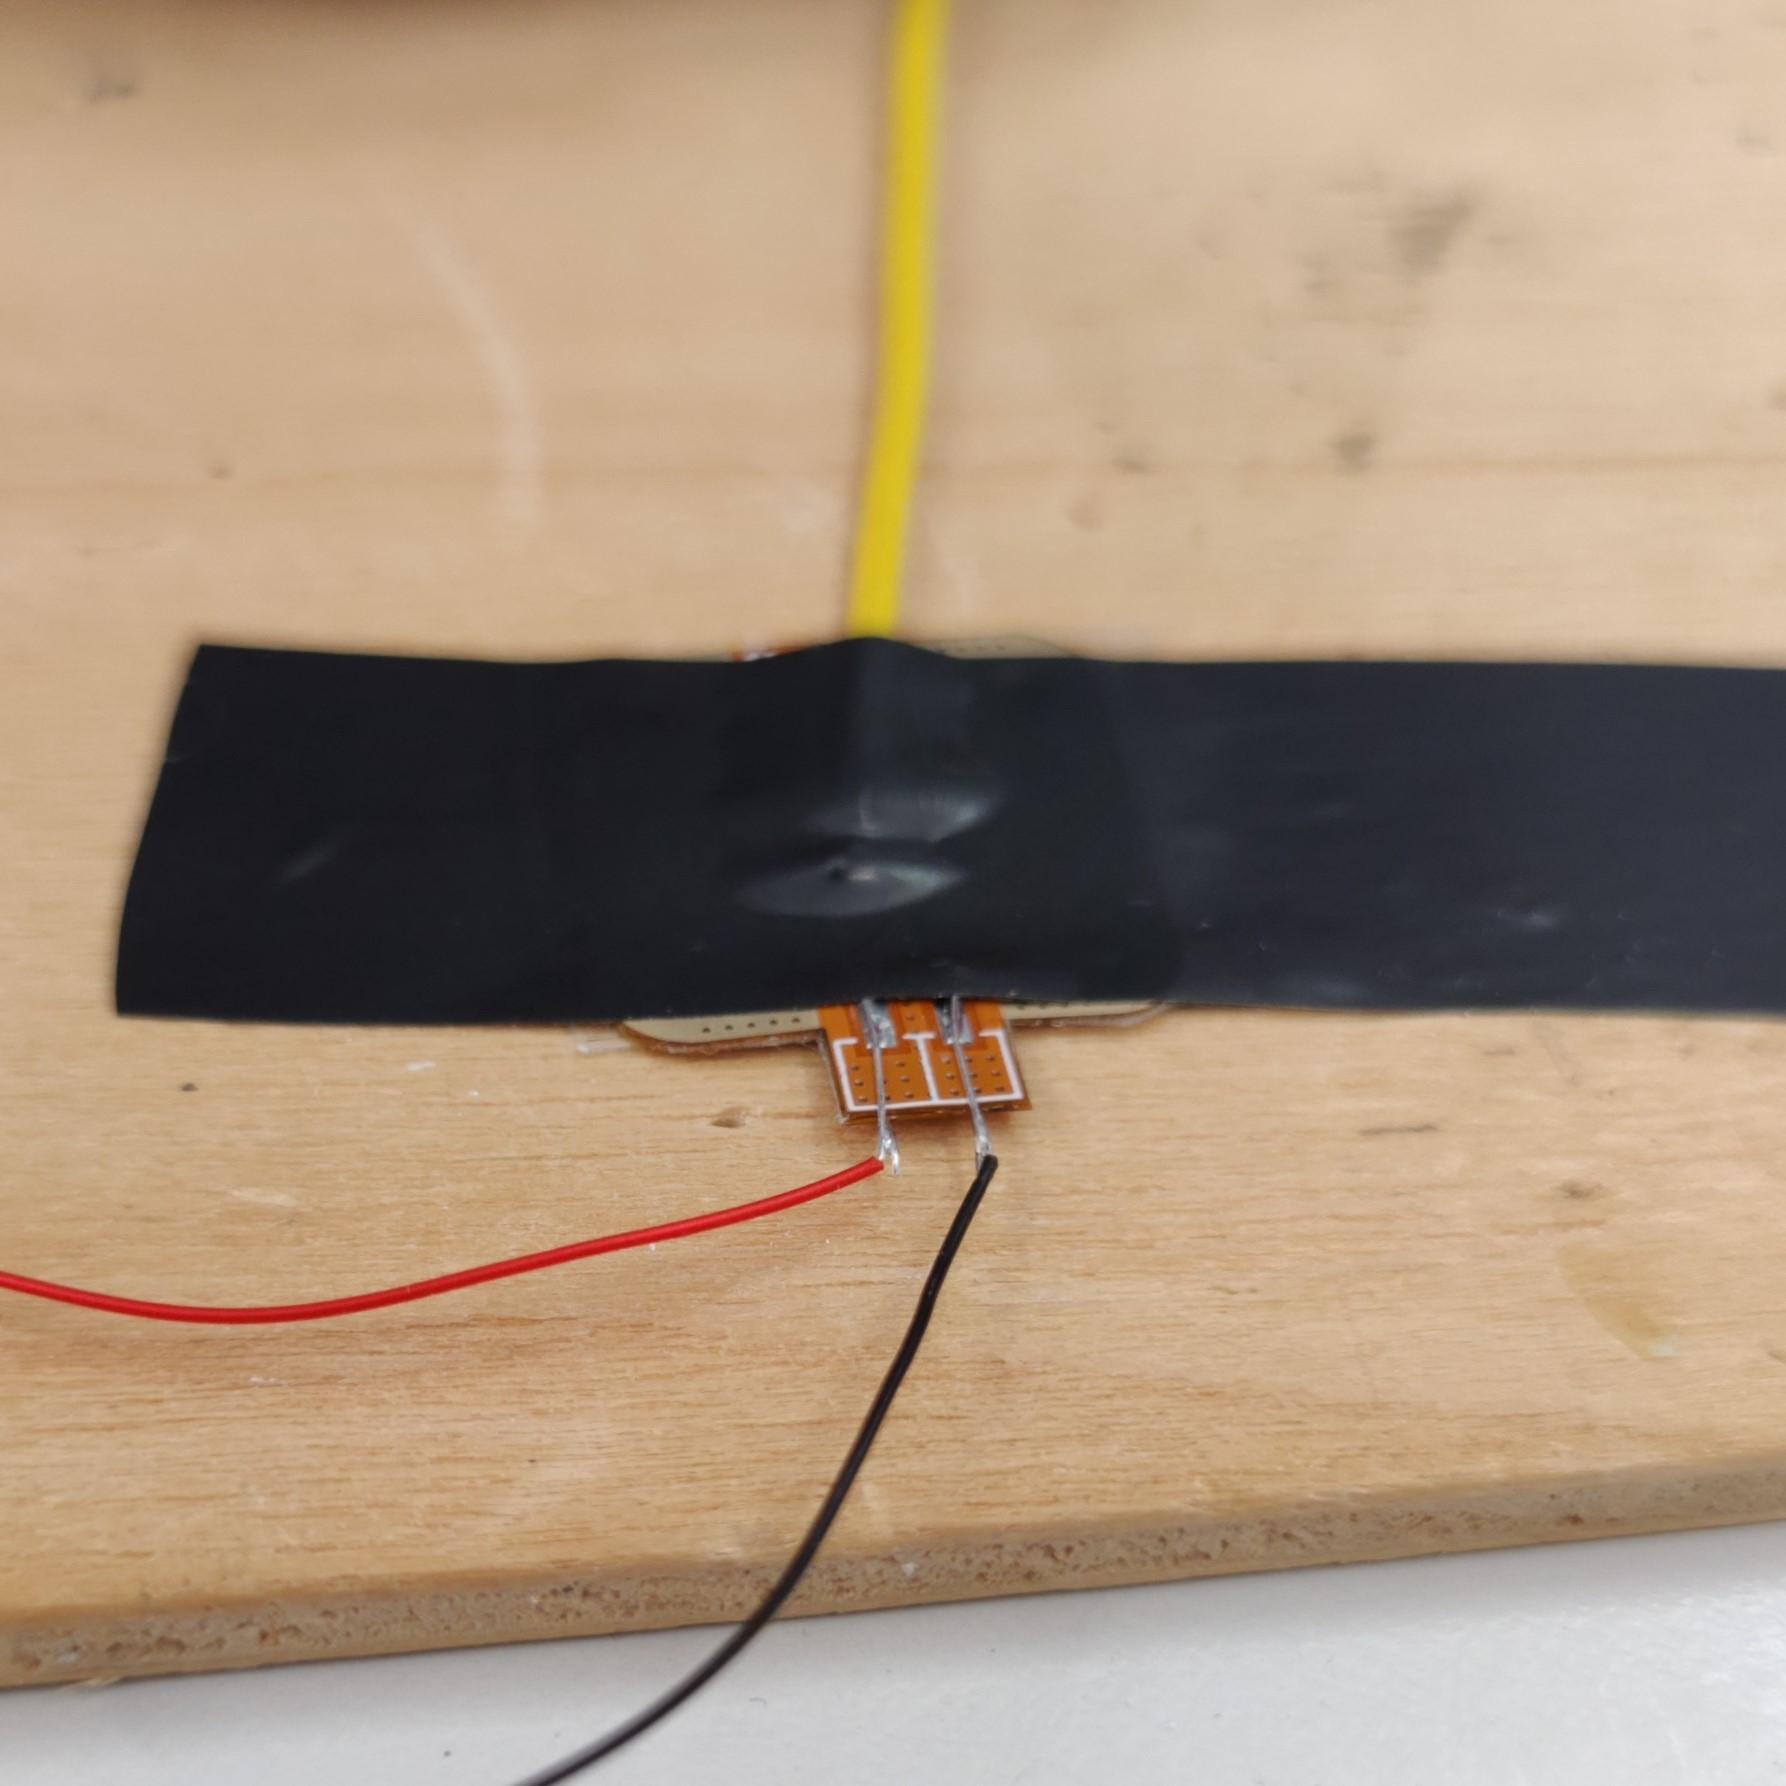
\includegraphics{Chapters/Chapter5/Exp_Evaluation/Figures/Heating_test_setup.jpg}
    }
    \caption{Heating test setup.}
    \label{fig: Heating_test_setup}
\end{figure}

\subsubsection{Single coil tests' results}
The results of the single coil tests are shown in figure \ref{fig: Single_coil_heating_tests}.
\begin{figure}
    \centering
    \resizebox{0.9\textwidth}{!}{
        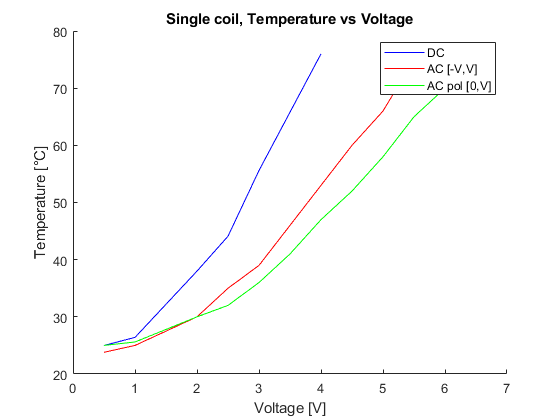
\includegraphics{Chapters/Chapter5/Exp_Evaluation/Figures/Temp_vs_Volt_1_coil.png}
    }
    \caption{Temperature vs Voltage for one coil.}
    \label{fig: Single_coil_heating_tests}
\end{figure}
As we can observe the coil tends to heat up way less in AC conditions, especially in the unipolar case.
This is due to the lower RMS value of the current that flows through the coil in AC conditions.

\subsubsection{Two coils in parallel tests' results}
The results of the two coils in parallel tests are shown in figure \ref{fig: Two_coils_heating_tests}.
\begin{figure}
    \centering
    \resizebox{0.9\textwidth}{!}{
        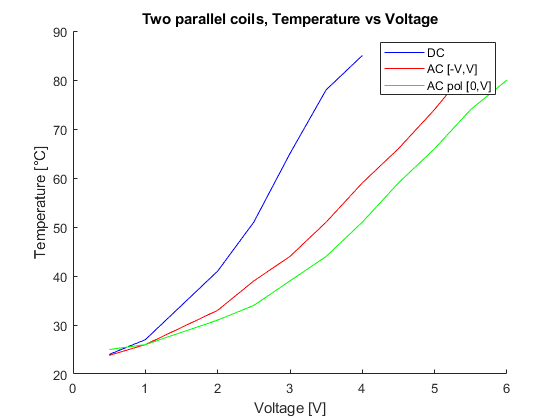
\includegraphics{Chapters/Chapter5/Exp_Evaluation/Figures/Temp_vs_Volt_2_coils.png}
    }
    \caption{Temperature vs Voltage for two coils in parallel.}
    \label{fig: Two_coils_heating_tests}
\end{figure}
This case is comparable to the previous one, but here the two coils in parallel tend to heat up more than the single coil even if the current is divided between the two coils.
This is because the two coils are glued together and the heat generated by one coil is transferred to the other one.

% -- Subsection 4.3
\subsection{Force testing}
The force testing was conducted on the flexible mat prototypes.
The goal of these tests was to understand the relationship between the force generated by the coil and the voltage applied to it.
To measure the force generated by the coil we used an ATI TW-Nano17 force sensor.
As we needed to measure the force in the z direction we had to create a way to suspend the sensor above the mat membrane.
This mount should also allow the sensor's position to be adjusted on the z-axis to be able to position the sensor at the right height to not press the membrane too much.
We modeled the structure based on the 3D model of the ATI sensor and then 3D printed its various components.

\begin{figure}
    \centering
    \resizebox{0.9\textwidth}{!}{
        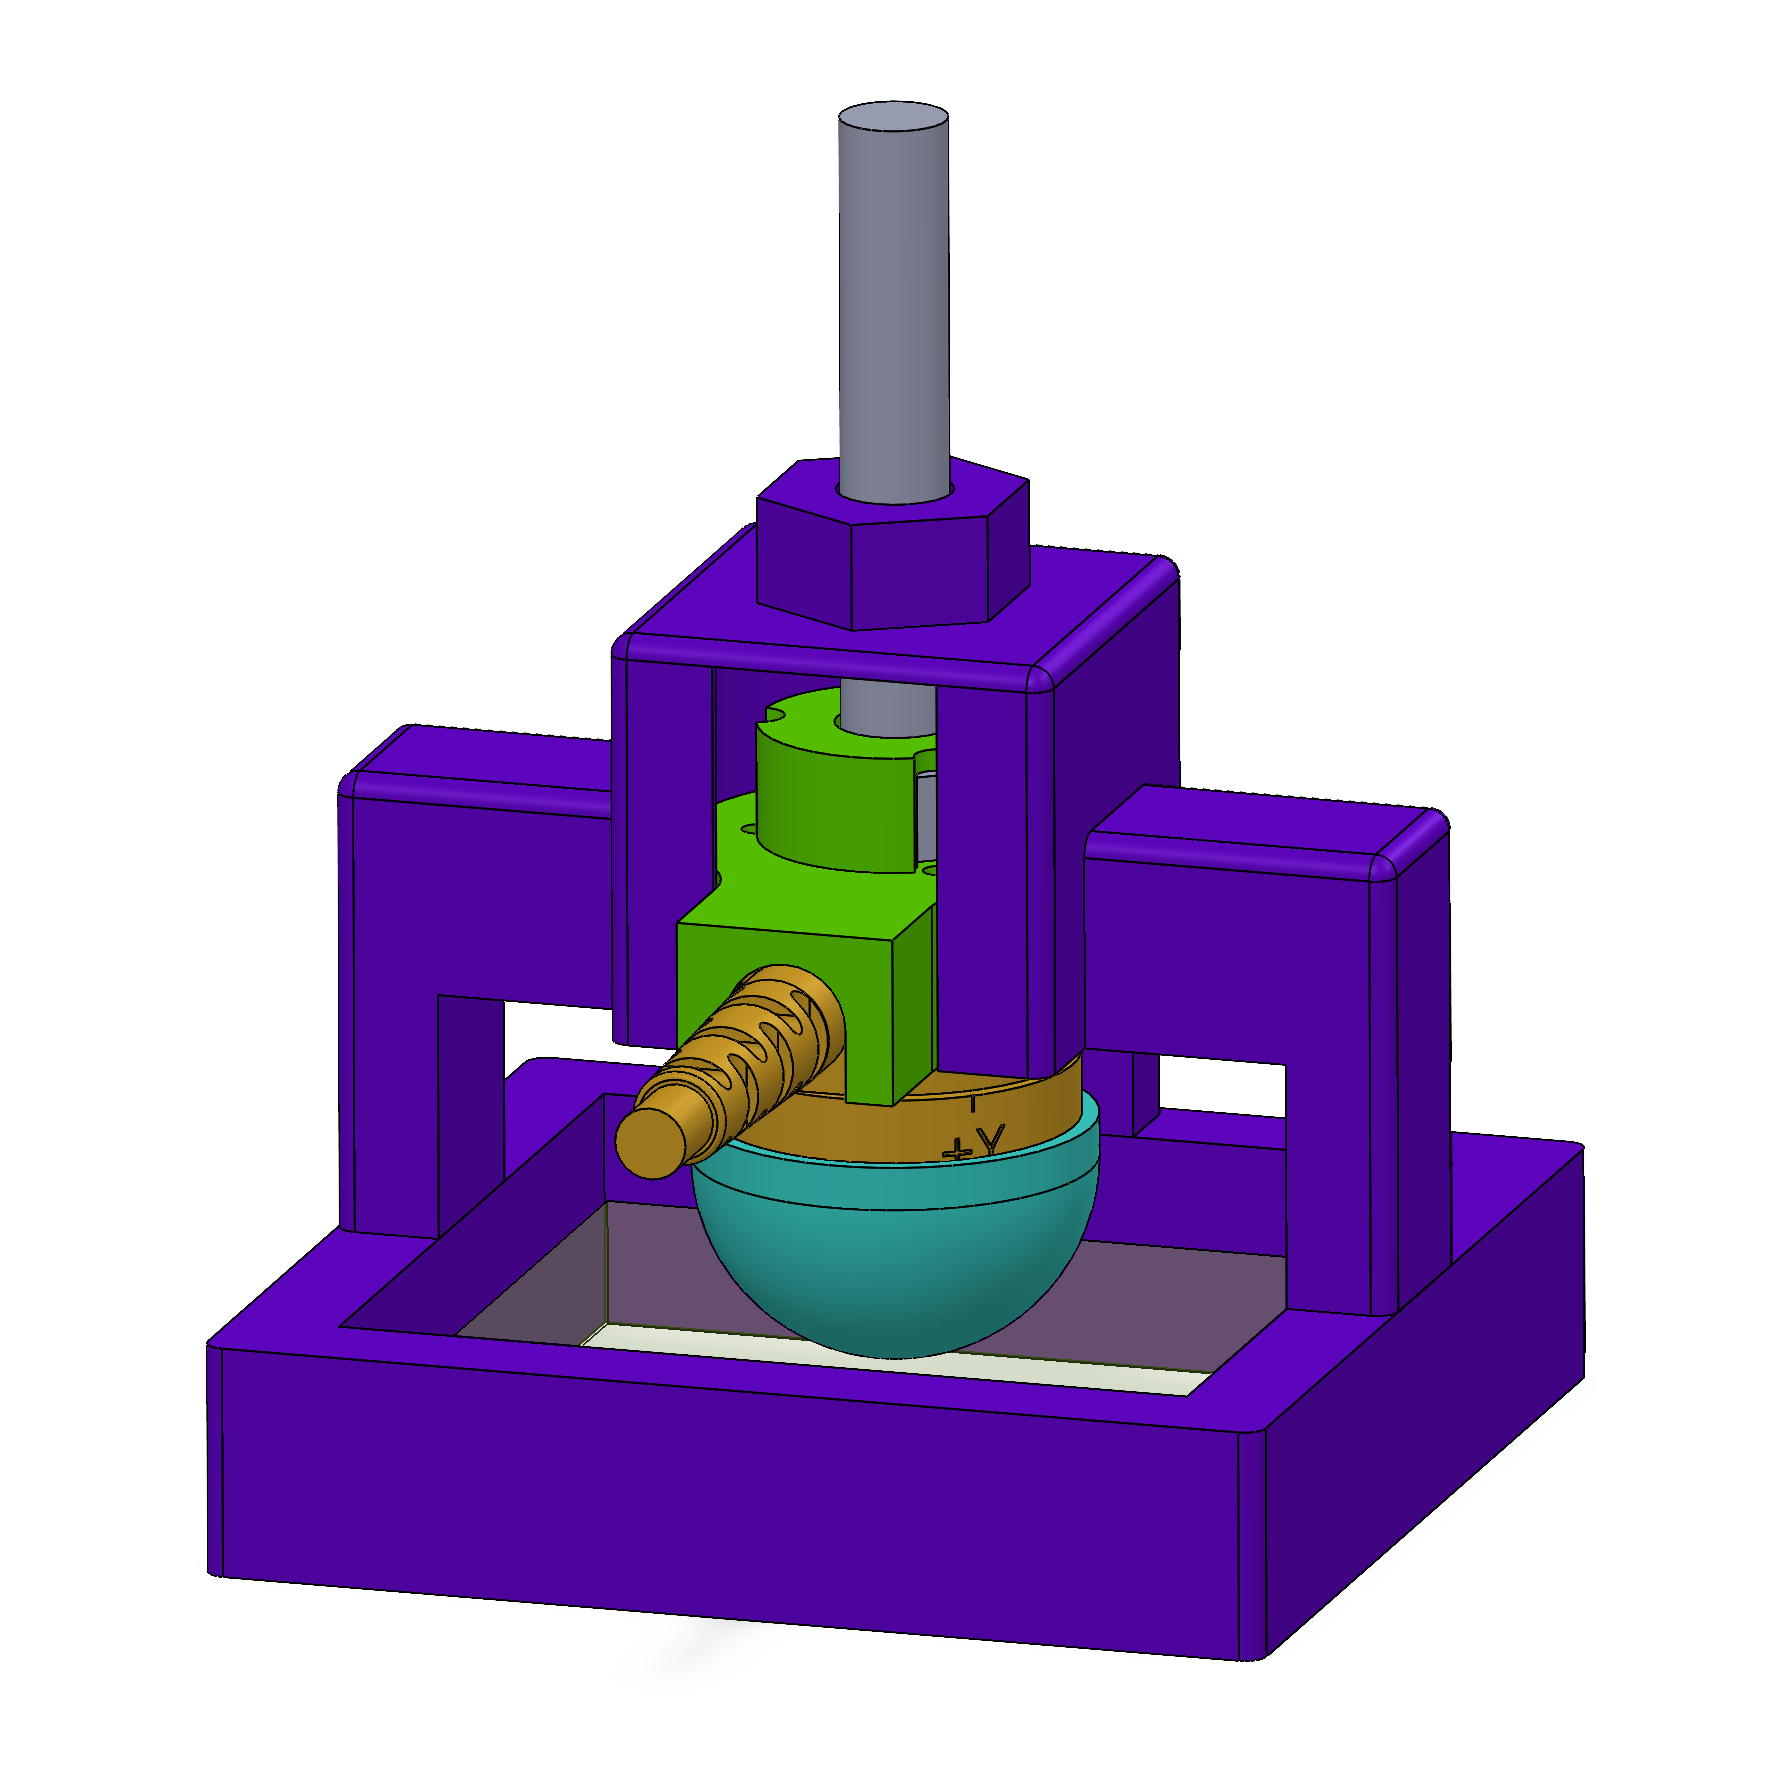
\includegraphics{Chapters/Chapter5/Exp_Evaluation/Figures/ATI_test_platform.png}
    }
    \caption{Sensor mount complete structure.}
    \label{fig: Sensor_mount_complete}
\end{figure}

The structure is composed of 3 3D printed PLA components, one nut and a bolt.
The components are the following:
\begin{itemize}
    \item \textbf{Sensor mount:} this component holds the sensor and houses the bolt head on its top. It was designed to trap the head of the bolt but to leave it able to rotate, this was done by temporarily pausing the printing process and inserting the bolt. Then the printing process was resumed to create the blocking layers on the bottom of the bolt's head. (Green component in figure \ref{fig: Sensor_mount_complete})
    \begin{figure}
        \centering
        \resizebox{0.9\textwidth}{!}{
            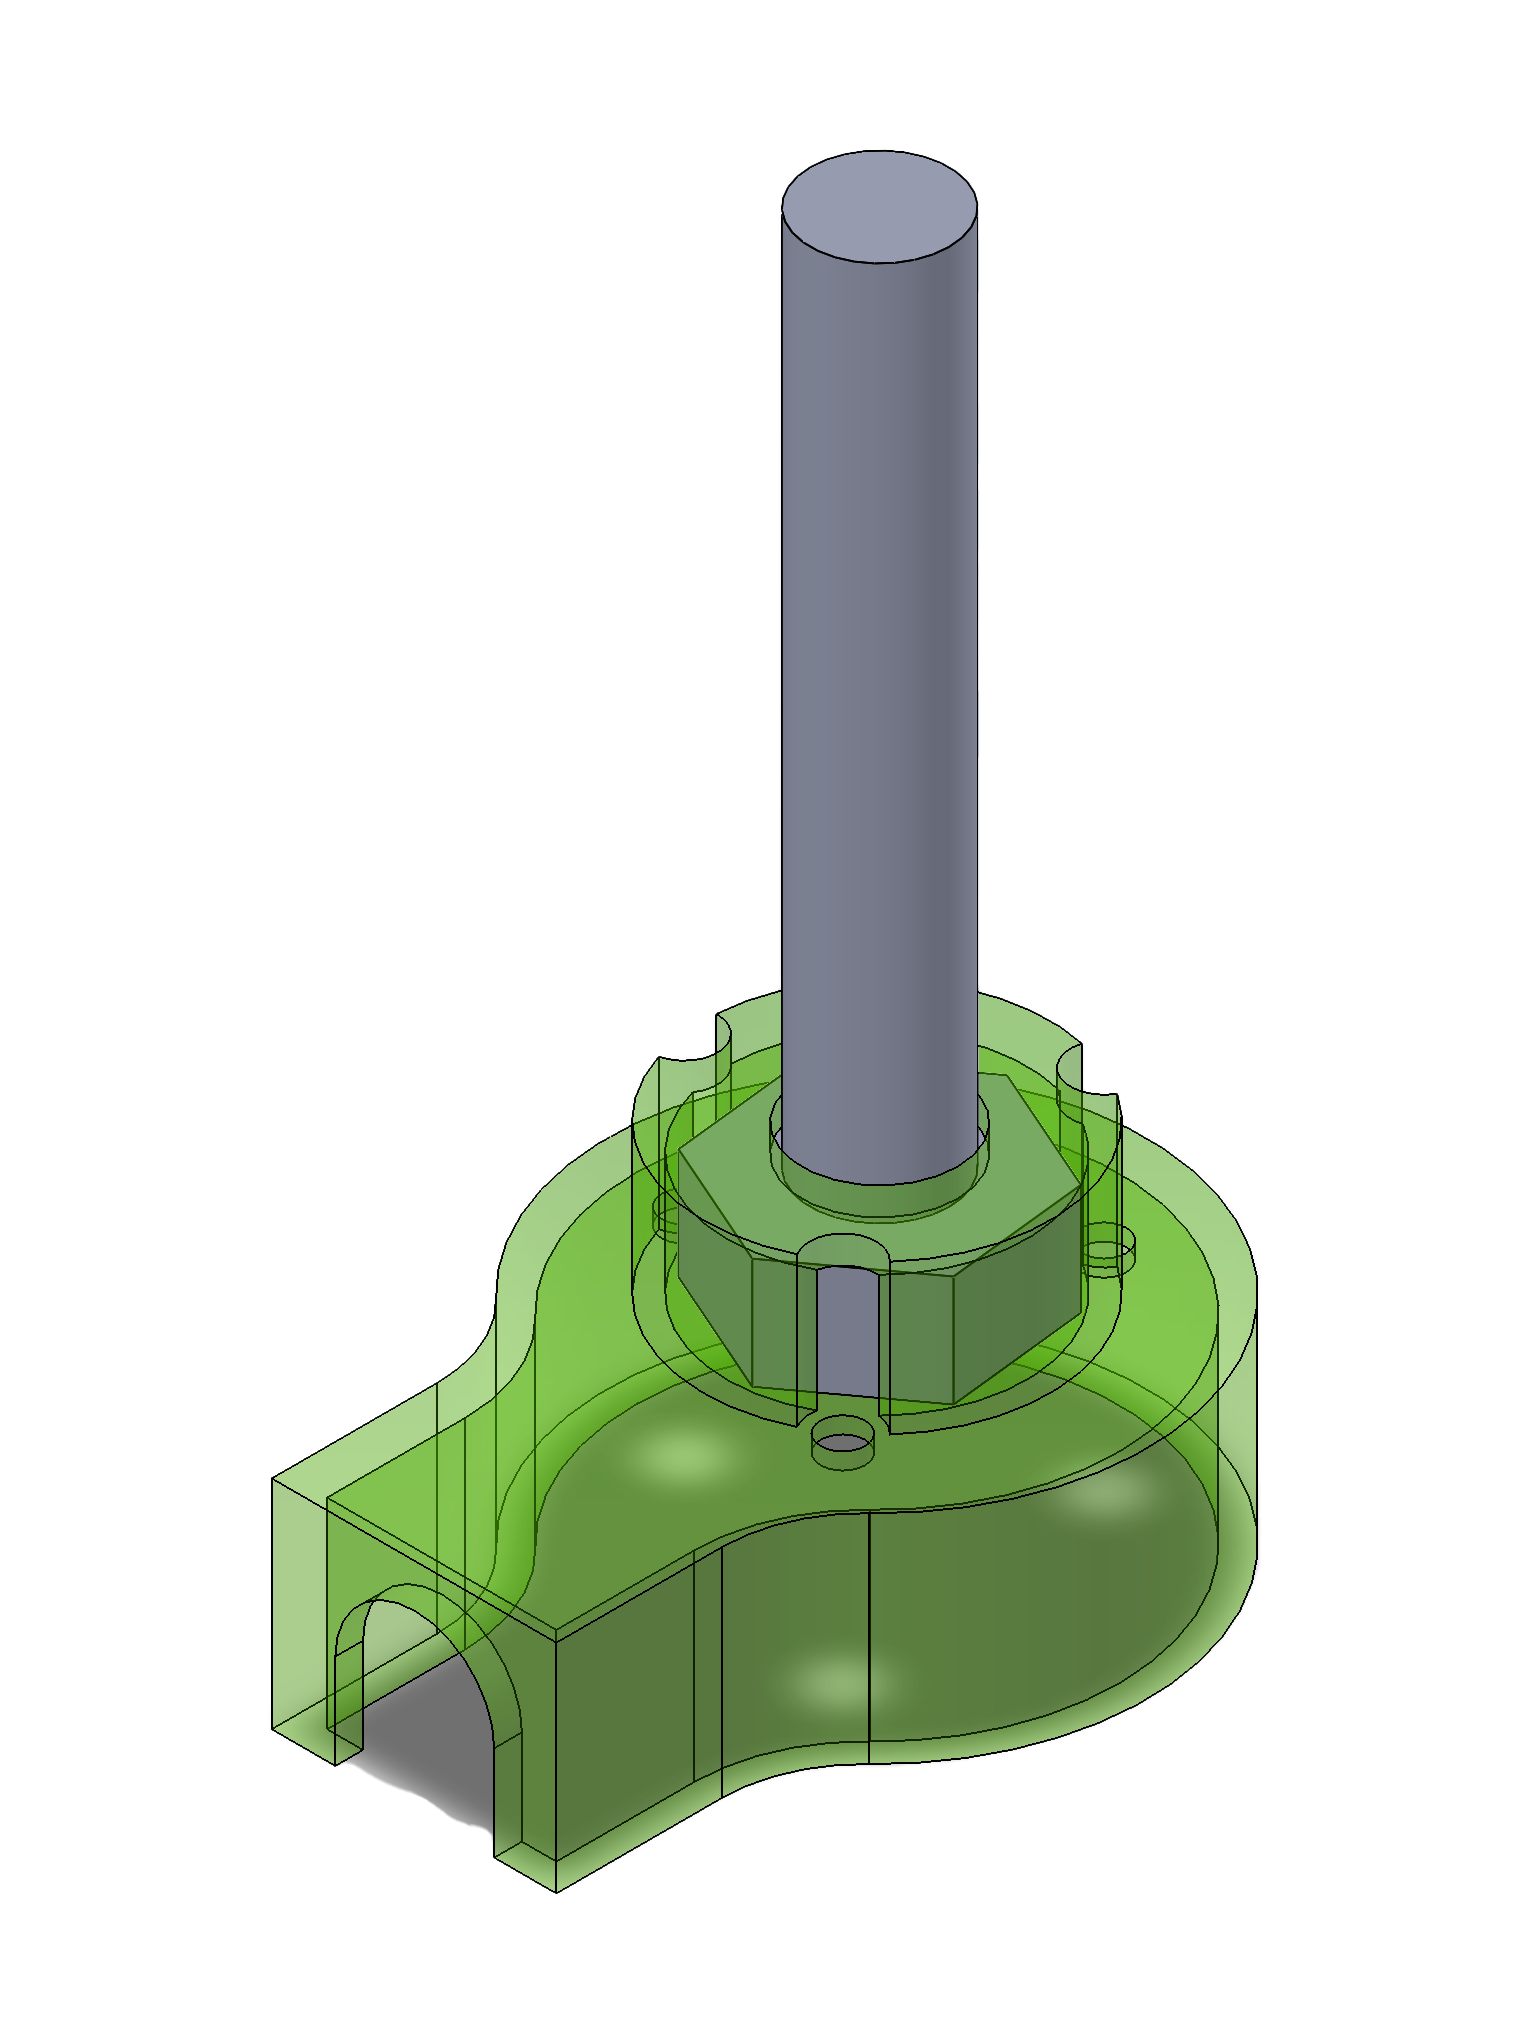
\includegraphics{Chapters/Chapter5/Exp_Evaluation/Figures/ATI_grabber.png}
        }
        \caption{Sensor mount see-through view.}
        \label{fig: Sensor_mount}
    \end{figure}

    \item \textbf{Sensor mount base:} this component is the base of the structure, on the bottom has a squared hole where the flexible mat can be inserted and on the top houses a nut trapped in the print to allow the bolt to be screwed up and down. (Purple component in figure \ref{fig: Sensor_mount_complete})
    \begin{figure}
        \centering
        \resizebox{0.9\textwidth}{!}{
            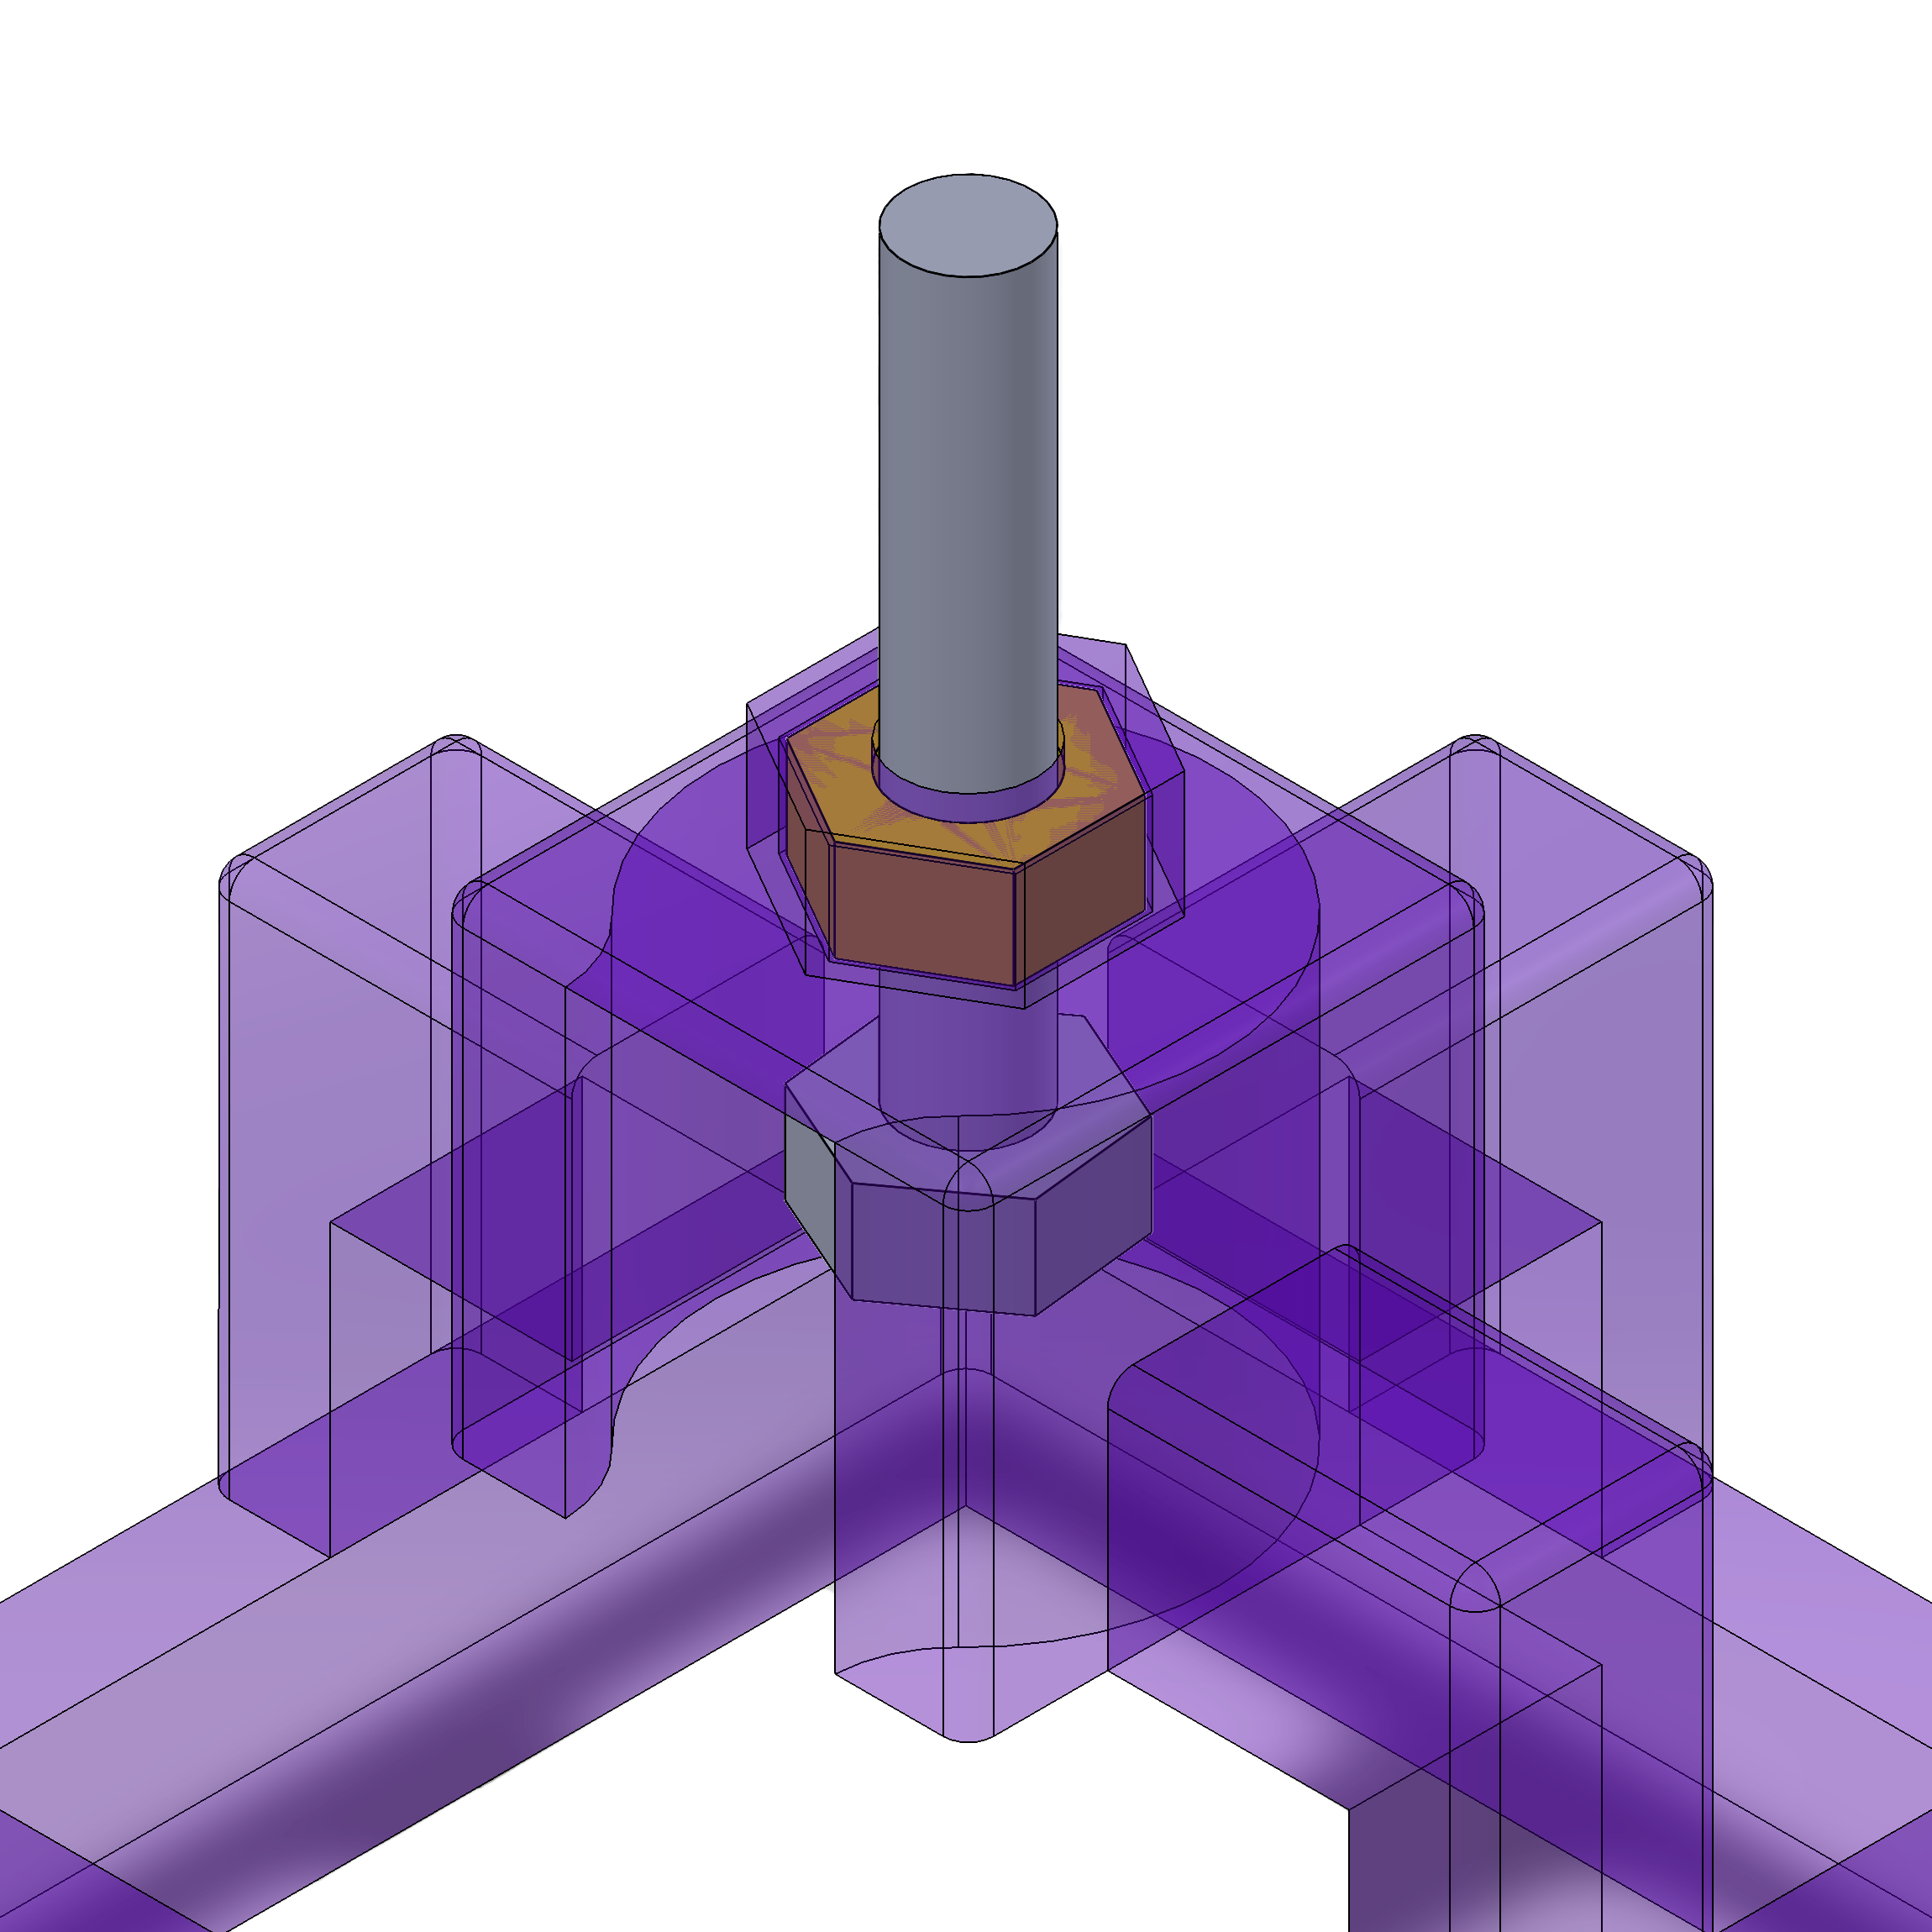
\includegraphics{Chapters/Chapter5/Exp_Evaluation/Figures/ATI_platform_mech.png}
        }
        \caption{Sensor mount base see-through view of the nut and bolt mechanism.}
    \end{figure}

    \item \textbf{Sensor's pulp:} this component is mounted below the sensor and is used to press the membrane of the mat on a small area, to simulate a finger pressing on the mat. (Teal component in figure \ref{fig: Sensor_mount_complete})

\end{itemize}

The complete test setup is shown in figure \ref{fig: Force_test_setup}.
\begin{figure}
    \centering
    \resizebox{0.9\textwidth}{!}{
        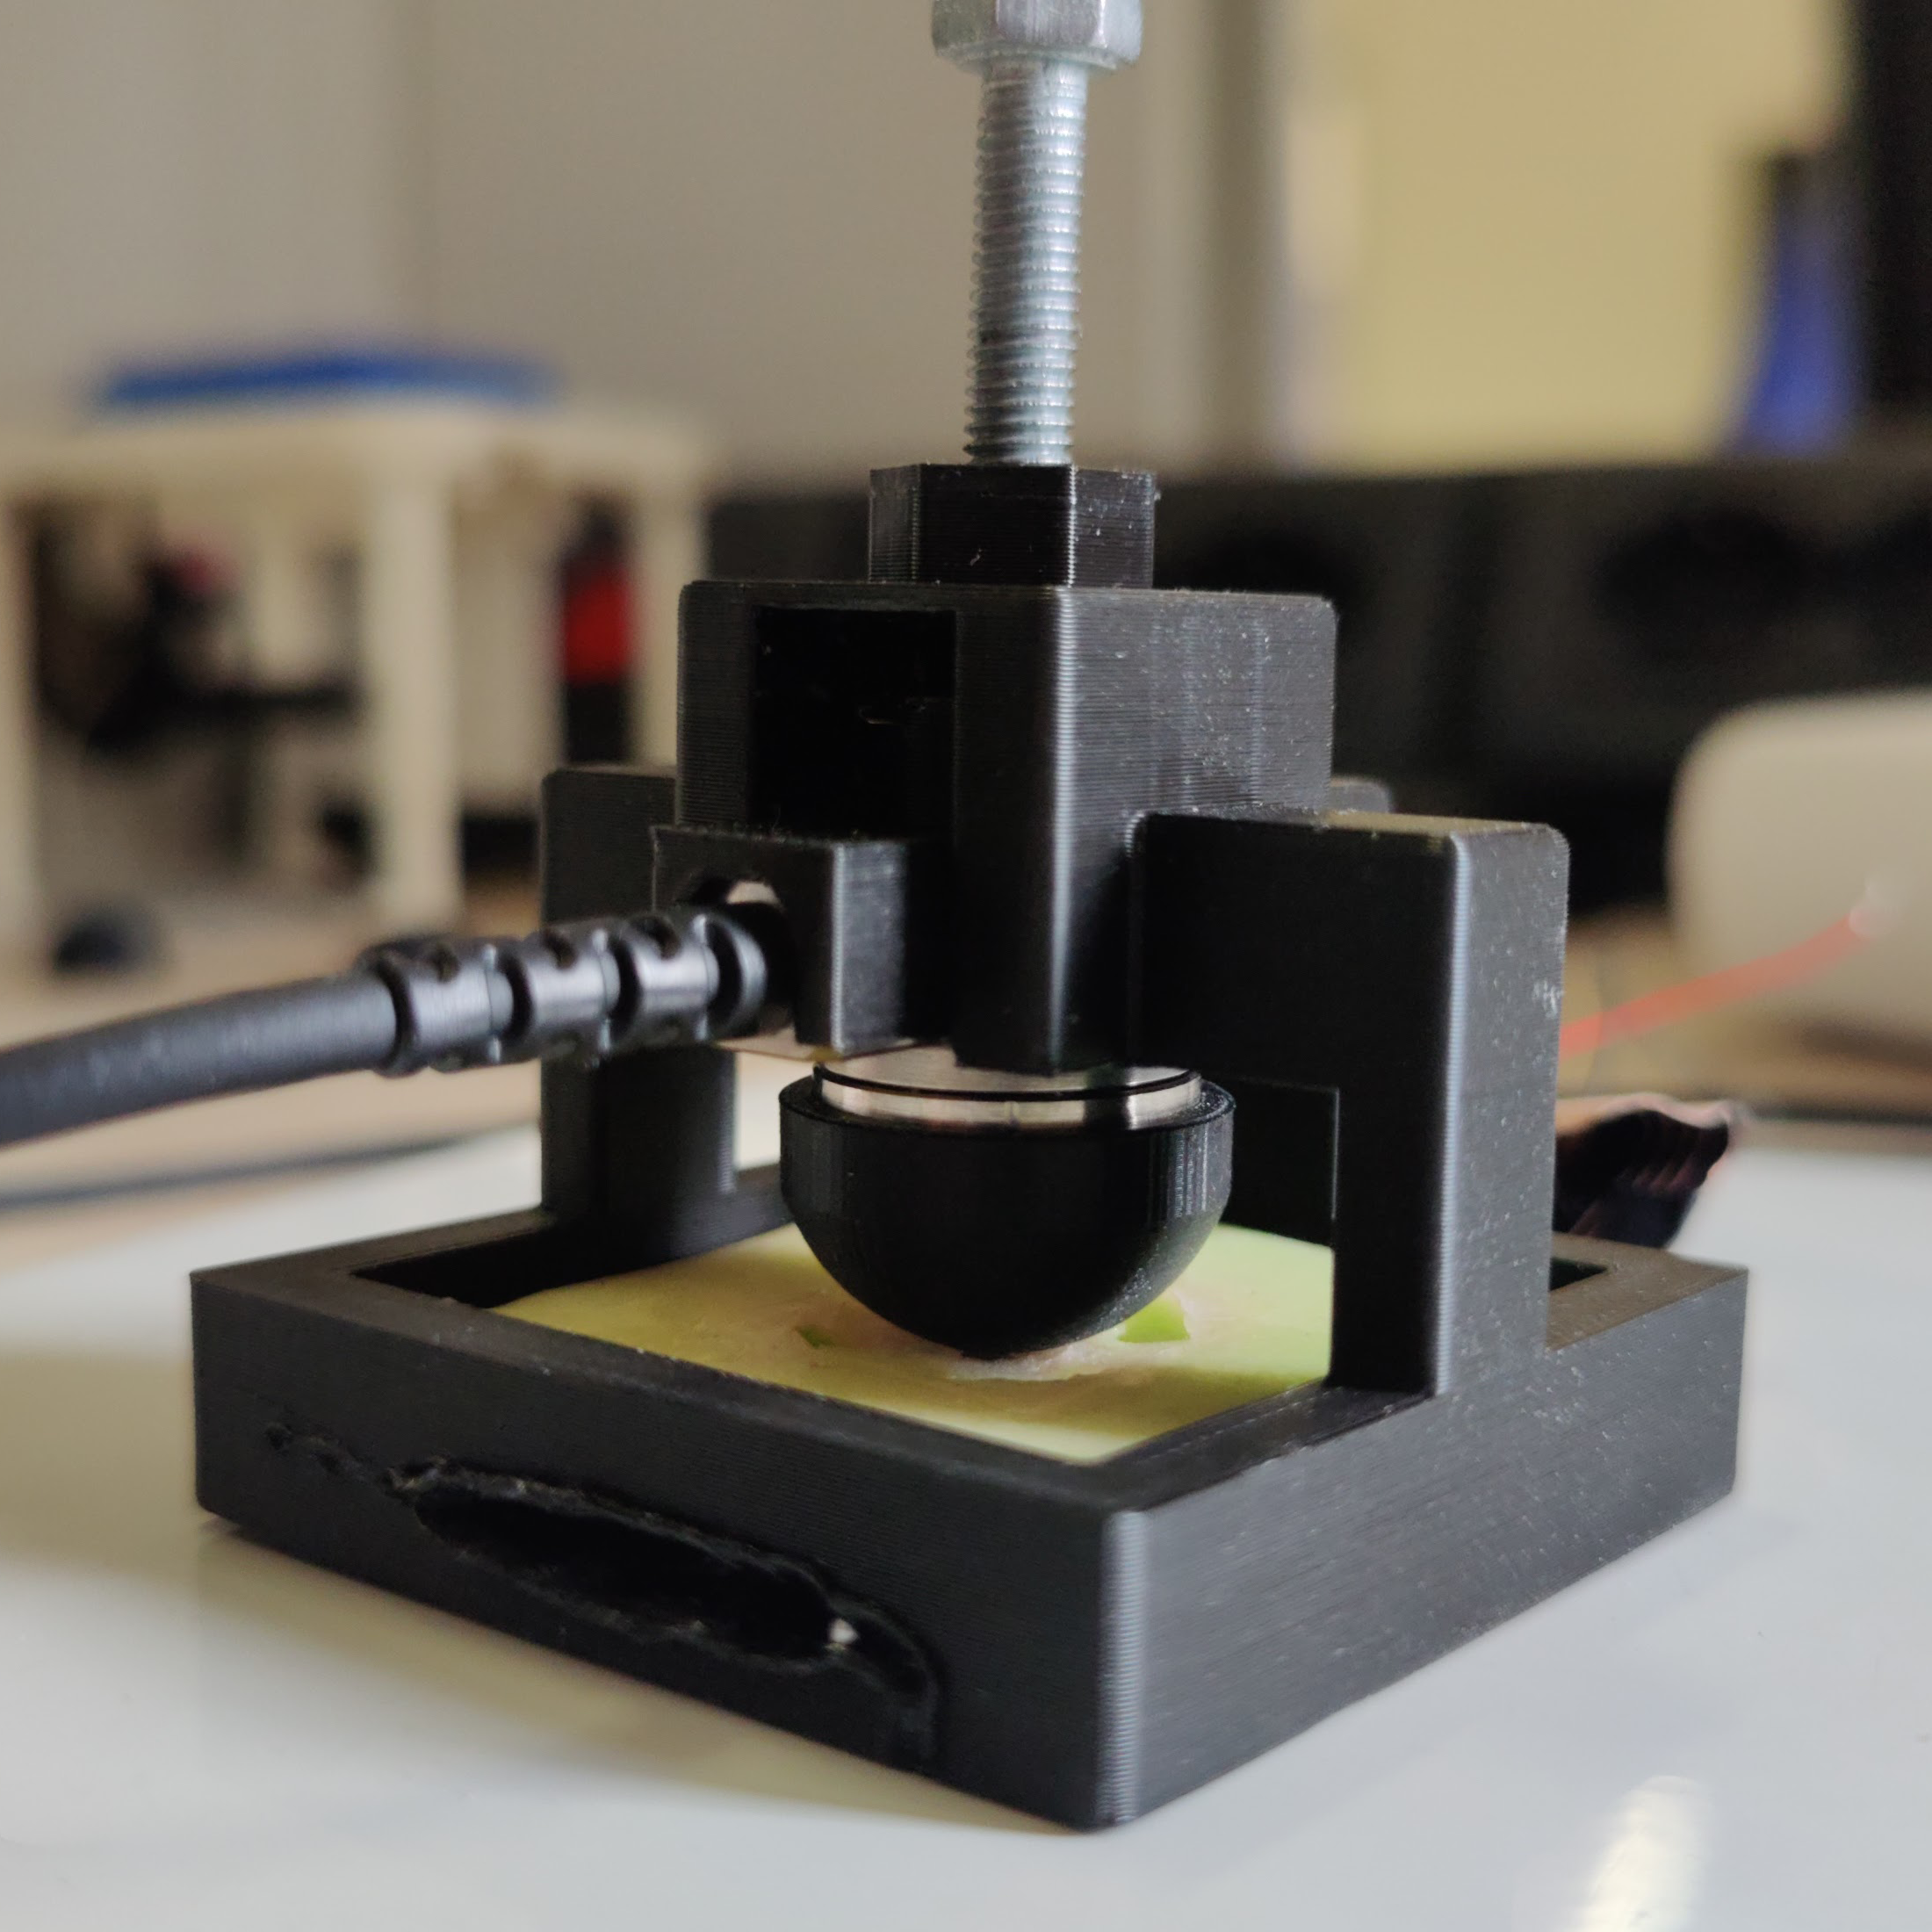
\includegraphics{Chapters/Chapter5/Exp_Evaluation/Figures/ATI_mat_complete.png}
    }
    \caption{Complete force testing setup.}
    \label{fig: Force_test_setup}
\end{figure}

ATI data acquisition was done with a MATLAB script based on the work of \cite{ATI_NetFT_MatlabInterface}.

\subsubsection{ATI sensor low sensitivity}
After some tests, we quickly realized that the ATI sensor was not sensitive enough to measure the forces generated by the mat prototype when driven with sinusoidal signals.
This is because, even at the max rated voltage we can drive the coil with (6V), the magnetic field generated by the coil is not strong enough to generate a magnetic repulsion force with the magnet that can be measured by the sensor.
The only way to measure the force generated by the coil is to make it produce a way higher magnetic field, the solution we found was to use a signal with very high peaks but low RMS voltage.
In this way, the coil can generate high peaks of magnetic field for a short time, enough to generate a force that can be measured by the sensor.
A good candidate for testing with this type of signals is the heartbeat pulse, it presents a very high peak at the ventricles contraction and then a low value during the rest of the heartbeat cycle.
\begin{figure}
    \centering
    \resizebox{0.9\textwidth}{!}{
        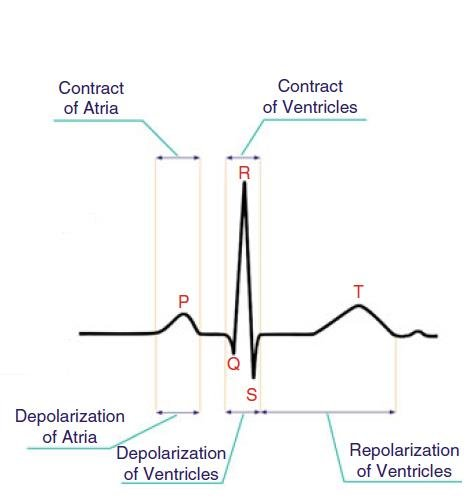
\includegraphics{Chapters/Chapter5/Exp_Evaluation/Figures/heartbeat_pulse.png}
    }
    \caption{Heartbeat pulse.}
    \label{fig: Heartbeat_pulse}
\end{figure}
We chose the heartbeat because it's a good example for our case study as it is a low-frequency signal and because we managed to run the coil with it even at up to 30V peak value without reaching its thermal runaway point.
Also, the simulated heartbeat was easily recognizable by the subjects who tested the flexible mat prototype.

\subsubsection{Testing procedure}
To measure the force generated by the mat prototypes we used an automatic testing procedure controlled by a MATLAB script.
The computer running the script was connected to the function generator and the ATI sensor.
The script was designed to:
\begin{itemize}
    \item Set the function generator to output the desired signal, voltage and frequency.
    \item Measure the force offset on the sensor when the coil was off.
    \item Turn on the signal on the function generator.
    \item Read the sensor data for a given amount of seconds, with a given number of samples.
    \item Turn off the signal.
\end{itemize}
Then the script would plot the force data and save it to a file.

\subsubsection{Magnet size vs Force}
The main reason we decided to carry out this test was to compare the force generated by the two mat prototypes we developed, the one with the small magnet and the one with the big magnet.
We tested them both using two coils in parallel and the heartbeat pulse signal at 30V peak value.

The results of the tests are shown in figure \ref{fig: Force_vs_magnet_size}.
\begin{figure}
    \centering
    \begin{subfigure}[b]{0.475\textwidth}
        \centering
        \resizebox{0.9\textwidth}{!}{
            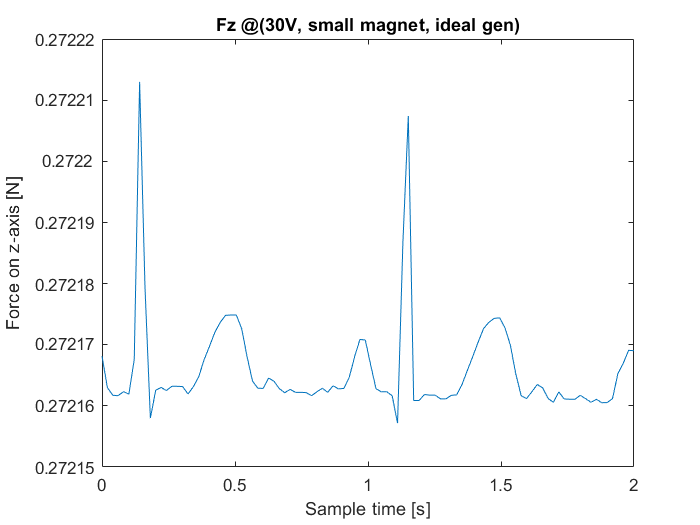
\includegraphics{Chapters/Chapter5/Exp_Evaluation/Figures/Fz_@30V_small_magn_idealgen.png}
        }
        \caption{Force profile of the small magnet prototype.}
    \end{subfigure}
    \begin{subfigure}[b]{0.475\textwidth}
        \centering
        \resizebox{0.9\textwidth}{!}{
            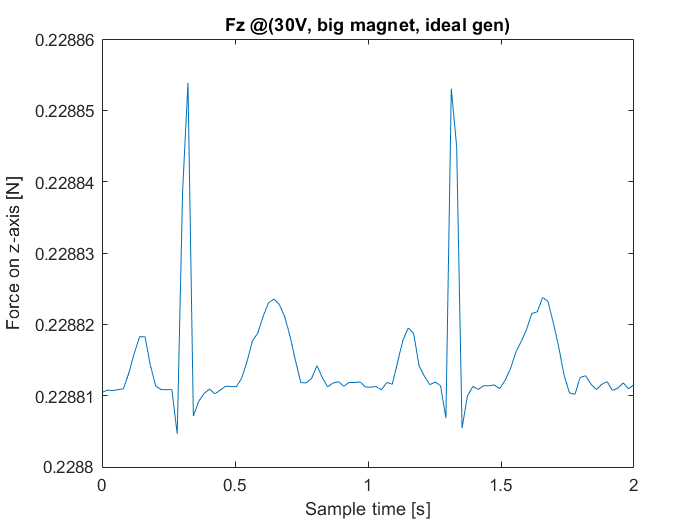
\includegraphics{Chapters/Chapter5/Exp_Evaluation/Figures/Fz_@30V_big_magn_idealgen.png}
        }
        \caption{Force profile of the big magnet prototype.}
    \end{subfigure}
    \caption{Force profile of the two mat prototypes run with the heartbeat pulse signal.}
    \label{fig: Force_vs_magnet_size}
\end{figure}

As we can see the force generated by the two prototypes is comparable, but sadly the force generated by the big magnet prototype is lower than the one generated by the small magnet prototype.

